\documentclass[11pt,a4paper,parskip=half]{scrartcl}
\usepackage[T1]{fontenc}
\usepackage[utf8]{inputenc}
%\usepackage{tgpagella}
\usepackage{tgheros} % TeX Gyre Heros (sans-serif for headings)
\usepackage[bitstream-charter]{mathdesign} % Bitstream Charter (for text)
\usepackage[bf,sf]{titlesec} % not needed atm?
\usepackage[protrusion=true,expansion=true]{microtype} % "beautification"
\usepackage{geometry}
\geometry{left=2.5cm,right=2.5cm,bottom=4cm,top=3cm}

\usepackage{caption}
\usepackage{subcaption}
\usepackage{etoolbox}
\usepackage{fancyhdr}
%\usepackage{enumerate}
\usepackage{enumitem}
\usepackage{booktabs}
\usepackage[usenames,dvipsnames]{xcolor}
\usepackage{wrapfig}
\usepackage{url}
%\usepackage{gb4e}
\usepackage{covington}
\usepackage{ngerman}
\usepackage{tikz}
\usepackage[framemethod=tikz]{mdframed}
\usepackage{graphicx}
\usepackage{overpic}

\newtoggle{usenorm}
\toggletrue{usenorm}

\begin{document}

\newcommand{\mmb}{Marcel Bollmann ({\small\url{bollmann@linguistics.rub.de}})}
\newcommand{\trans}[1]{"`{\small\texttt{#1}}"'}
\newcommand*\circled[1]{\tikz[baseline=(char.base)]{\node[shape=circle,draw,inner sep=1pt,fill=yellow] (char) {\small\textbf{#1}};}}

%%%%%%%%%%%%%%%%%%%%%%%%%%%%%%%%%%%%%%%%%%%%%%%%%%
%%%% DEFINITION OF BOX ENVIRONMENTS %%%%%%%%%%%%%%
%%%%%%%%%%%%%%%%%%%%%%%%%%%%%%%%%%%%%%%%%%%%%%%%%%

\newenvironment{infobox}[1]{
  \begin{mdframed}[linewidth=1,leftmargin=20,rightmargin=20,%
    backgroundcolor=Yellow!50,linecolor=GreenYellow,%
    splittopskip=\topskip,skipbelow=0.5\baselineskip,%
    skipabove=\baselineskip,%
    roundcorner=6pt,%
    innerleftmargin=6pt,innerrightmargin=6pt,%
    innerbottommargin=.85\baselineskip,innertopmargin=6pt]
    \textbf{#1}\\
}{
  \end{mdframed}
}

\newenvironment{alertbox}[1]{
  \begin{mdframed}[linewidth=1,leftmargin=20,rightmargin=20,%
    backgroundcolor=Red!45,linecolor=Sepia,%
    splittopskip=\topskip,skipbelow=0.5\baselineskip,%
    skipabove=\baselineskip,%
    roundcorner=6pt,%
    innerleftmargin=6pt,innerrightmargin=6pt,%
    innerbottommargin=.85\baselineskip,innertopmargin=6pt]
    \textbf{#1}\\
}{
  \end{mdframed}
}

%%%%%%%%%%%%%%%%%%%%%%%%%%%%%%%%%%%%%%%%%%%%%%%%%%
%%%% TITLE AND PAGE STYLES %%%%%%%%%%%%%%%%%%%%%%%
%%%%%%%%%%%%%%%%%%%%%%%%%%%%%%%%%%%%%%%%%%%%%%%%%%

\pagestyle{fancy}
\lhead{\emph{CorA Benutzerhandbuch}}
%\rhead{108004242751 $\cdot$ Bollmann}

%\originalTeX

\title{CorA (Corpus Annotator)\\Benutzerhandbuch}
\subtitle{Version 1.2} \author{Marcel
  Bollmann\\\url{bollmann@linguistics.rub.de}\\Sprachwissenschaftliches
  Institut\\Ruhr-Universität Bochum} \date{\today}
\maketitle

%\setcounter{page}{1}
\tableofcontents
\newpage

%%%%%%%%%%%%%%%%%%%%%%%%%%%%%%%%%%%%%%%%%%%%%%%%%%
%%%% CONTENT %%%%%%%%%%%%%%%%%%%%%%%%%%%%%%%%%%%%%
%%%%%%%%%%%%%%%%%%%%%%%%%%%%%%%%%%%%%%%%%%%%%%%%%%

\section{Allgemeines}

CorA ist ein web-basiertes Programm zur Annotation von Korpora.  Die
aktuelle Adresse~(URL) von CorA lautet:

\begin{quote}
  \url{http://smokehead.linguistics.rub.de/cora/}
\end{quote}

Wir empfehlen die Verwendung einer aktuellen Version von Google
Chrome\footnote{\url{http://www.google.com/chrome/}} (bzw.\ Chromium)
oder Mozilla Firefox\footnote{\url{http://www.mozilla.com/}}.
JavaScript darf nicht deaktiviert sein.  CorA funktioniert
möglicherweise auch mit anderen Browsern, jedoch wird das Tool von uns
nur mit den genannten Browsern getestet.

\begin{alertbox}{Wichtig!}
  Die Benutzung von CorA erfordert eine ständige Internetverbindung.
  Es ist nicht möglich, das Tool offline zu benutzen.  Wenn Sie
  während der Bearbeitung eines Dokuments länger als 30~Minuten
  offline sind, kann ein Datenverlust nicht ausgeschlossen werden.
\end{alertbox}

Bitte öffnen Sie CorA \textbf{nicht} gleichzeitig in mehreren
Browserfenstern auf demselben Rechner, und loggen Sie sich
\textbf{nicht} gleichzeitig mit demselben Benutzerkonto auf mehreren
Rechnern ein.  Dies kann zu unvorhergesehenem Verhalten führen, da
CorA hierfür nicht ausgelegt ist.

\subsection{Benutzername und Passwort}

Bevor Sie CorA benutzen können, müssen Sie sich mit Benutzernamen und
Passwort anmelden.  Falls ein neues Benutzerkonto angelegt werden
soll, oder Sie Ihr Passwort vergessen haben, wenden Sie sich bitte
direkt an \mmb{}.

Ihr \textbf{Passwort ändern} können Sie hingegen direkt in CorA:
hierzu loggen Sie sich zunächst ein, wechseln zum Reiter
"`Einstellungen"' und klicken dort auf die Schaltfläche "`Passwort
ändern\ldots"'.  Wenn Sie sich zum ersten Mal einloggen, sollten Sie
als erstes unbedingt Ihr Passwort ändern!

\subsection{Die Titelleiste}

In der Titelleiste, die sich immer am oberen Bildschirmrand befindet, können Sie

\begin{itemize}
\item Sigle und Dateinamen des aktuell geöffneten Dokuments sehen;
\item Benutzernamen und Online-Status sehen (das Symbol in der oberen rechten Ecke ist \textbf{grün,} wenn alles okay ist, und wird \textbf{rot,} falls die Verbindung zum Server verloren geht bzw.\ etwaige Fehler auftreten);
\item zwischen den verschiedenen Tabs wechseln (s.u.);
\item die aktuell geöffnete \textbf{Datei schließen} bzw.\ sich aus CorA \textbf{ausloggen.}
\end{itemize}

\newpage
\begin{figure}[!h]
  \centering
  \begin{overpic}[width=\linewidth]{img/1.2/header.png}
    %\put(2,32){\circled{1}}
  \end{overpic}
  \caption{Titelleiste von CorA}
  \label{fig:header}
\end{figure}

Hier eine Übersicht über die verschiedenen Tabs:

\begin{itemize}
\item \textbf{Datei:}  Hier können Dateien geöffnet, importiert, exportiert, oder gelöscht werden (s.\ Abschnitt~\ref{sec:datei}).
\item \textbf{Editor:}  Das Haupt-Editorfenster (s.\ Abschnitt~\ref{sec:editor}); nur sichtbar, wenn aktuell eine Datei geöffnet ist.
\item \textbf{Suchen:}  Hier erscheinen die Ergebnisse einer Suchanfrage (s.\ Abschnitt~\ref{sec:sufu}); nur sichtbar, nachdem eine Suchanfrage gestartet wurde.
\item \textbf{Einstellungen:}  Hier können Anpassungen am Editor vorgenommen werden (s.\ Abschnitt~\ref{sec:anpassen}).
\item \textbf{Hilfe:}  Hier findet sich u.a.\ immer die aktuellste Version dieses Benutzerhandbuchs.
\end{itemize}

\newpage
\section{Dateiverwaltung}
\label{sec:datei}

% \begin{figure}[!b]
%   \centering
% %  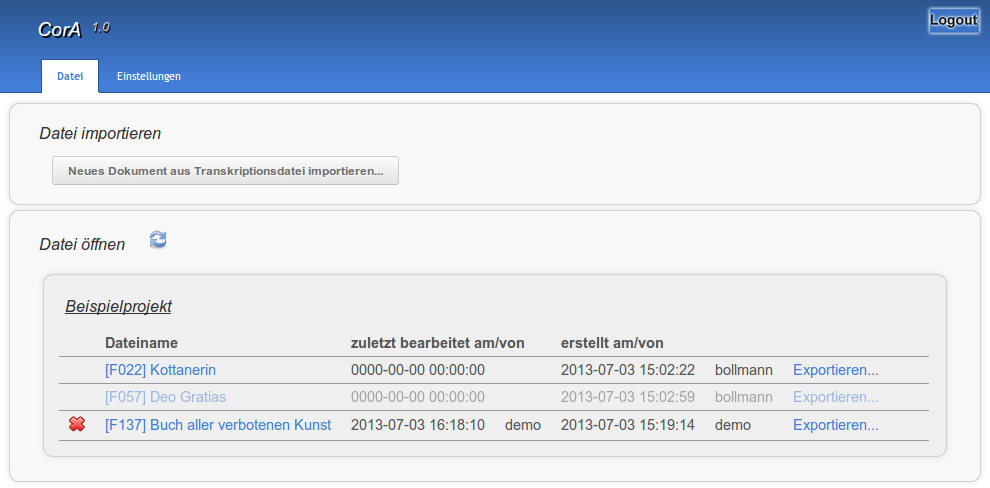
\includegraphics[width=\linewidth]{img/datei.png}
%   \begin{overpic}[width=\linewidth]{img/1.2/datei.png}
%     \put(2,32){\circled{1}}
%     \put(9,32){\circled{2}}
%     \put(13,32){\circled{3}}
%     \put(29,32){\circled{4}}
%     \put(3,25){\circled{5}}
%     \put(3,18){\circled{6}}
%     \put(94,22){\circled{7}}
%     \put(84,3){\circled{8}}
%   \end{overpic}
%   \caption{Dateien verwalten}
%   \label{fig:datei}
% \end{figure}

Nach der Anmeldung in CorA wird zunächst der Reiter "`Datei"' angezeigt:

\begin{figure}[!h]
  \centering
  \begin{overpic}[width=\linewidth]{img/1.2/datei.png}
    \put(2,32){\circled{1}}
    \put(9,32){\circled{2}}
    \put(13,32){\circled{3}}
    \put(29,32){\circled{4}}
    \put(3,25){\circled{5}}
    \put(3,18){\circled{6}}
    \put(94,22){\circled{7}}
    \put(84,3){\circled{8}}
  \end{overpic}
  \caption{Dateien verwalten}
  \label{fig:datei}
\end{figure}

Alle Dateien in CorA sind \textbf{Projekten} zugeordnet (hier
z.B. ``Beispielprojekt'').  Der Button \circled{1} aktualisiert die Dateiliste.
Ein Klick auf den Projektnamen klappt die Liste der zugeordneten Dateien ein
bzw.\ aus.  Die Buttons \circled{2} klappen die Dateilisten aller Projekte
gleichzeitig ein bzw.\ aus.

\textbf{Neue Texte importieren} können Sie entweder als Textdatei \circled{3}
oder als CorA-XML-Datei \circled{4}.  Der Import als Textdatei ist nur möglich,
wenn dem entsprechenden Projekt ein Importskript zugeordnet wurde, der das
Textformat intern nach CorA-XML konvertiert.  (Details zum Import finden sich in
Abschnitt \ref{sec:datei-import}.)

Die Dateien sind standardmäßig aufsteigend nach Sigle \textbf{sortiert} \circled{5}.
Durch Klick auf eine beliebige Spaltenüberschrift können Sie die Dateiliste nach
dieser Spalte sortieren lassen, um z.B.\ schnell alle kürzlich bearbeiteten
Dateien zu sehen.  Klicken Sie mehrmals auf dieselbe Spalte, um zwischen
aufsteigender und absteigender Sortierung zu wechseln.

Um eine Datei zu öffnen, klicken Sie einfach auf einen Dateinamen.  Dateien, die
\textbf{leicht ausgegraut} erscheinen \circled{6}, sind bereits von einem
anderen Nutzer geöffnet.  Eine Datei kann immer \textbf{nur von einem Nutzer
  gleichzeitig} geöffnet sein!  Klicken Sie den Dateinamen an, um zu erfahren,
wer die Datei aktuell geöffnet hat.  Die Datei kann erst wieder von jemand
anderem geöffnet werden, wenn dieser Nutzer die Datei schließt, sich ganz aus
CorA ausloggt, oder länger als 30~Minuten nicht mehr online gewesen ist.

\textbf{``Exportieren\ldots''} \circled{7} öffnet ein Fenster, um eine Datei im
CorA-XML-Format oder als mehrspaltige Textdatei zu exportieren.  Ein Klick auf
\circled{8} \textbf{löscht} eine Datei komplett; dieser Vorgang ist endgültig
und \textbf{kann nicht rückgängig gemacht werden!}  Nur Administratoren oder der
Benutzer, der die entsprechende Datei importiert hat, kann sie auch wieder
löschen.

%\begin{enumerate}[label=\protect\circled{\arabic*}]
%\item Aktualisiert die Dateiliste.
%\end{enumerate}

\subsection{Importieren von Transkriptionen}
\label{sec:datei-import}

\begin{figure}
  \centering
  \begin{subfigure}[b]{0.45\textwidth}
    \centering
    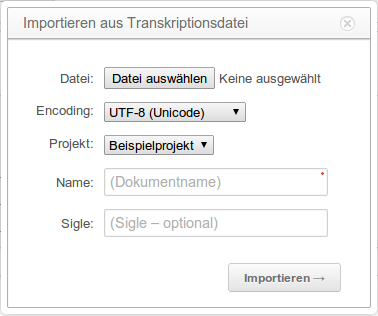
\includegraphics[width=\textwidth]{img/import-trans.png}
    \caption{Vor dem Import}
    \label{fig:import-dialog}
  \end{subfigure}
  \hfill
  \begin{subfigure}[b]{0.45\textwidth}
    \centering
    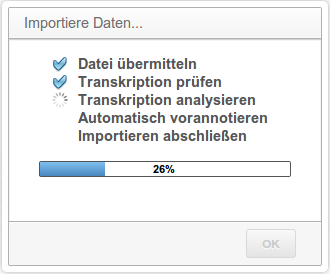
\includegraphics[width=\textwidth]{img/import-trans-progress.png}
    \caption{Während des Imports}
    \label{fig:import-progress}
  \end{subfigure}
  \caption{Importieren einer Datei}
  \label{fig:import}
\end{figure}

Neue Texte können jederzeit im CorA-XML-Format importiert werden.  Wenn für ein
Projekt ein Importskript festgelegt ist,\footnote{Dies können nur
  Administratoren einrichten.} können auch Textdateien, z.B.\
Transkriptionsdateien, direkt importiert werden via ``Import aus Textdatei''
(vgl.\ \circled{3} in Abbildung~\ref{fig:datei}).

Es öffnet sich ein Fenster ähnlich wie in
Abbildung~\ref{fig:import-dialog}.  Wählen Sie hier die \textbf{Datei}
aus, die Sie hochladen möchten, und geben Sie an in welchem
\textbf{Encoding} die Datei gespeichert wurde.  Stellen Sie ggf.\
sicher, dass das richtige \textbf{Projekt} ausgewählt ist (z.B.\
"`Referenzkorpus Frühneuhochdeutsch"').  Sie müssen außerdem
\textbf{Name} und \textbf{Sigle} des Dokuments angeben, unter denen es
in CorA geführt werden soll.

Der Import startet nach Klick auf "`Importieren"'.  Es öffnet sich ein
neues Fenster, welches den Fortschritt des Importvorgangs anzeigt
(Abbildung~\ref{fig:import-progress}).  Je nach Umfang der Datei kann
der Import \textbf{ca.\ 10~bis 15~Minuten} in Anspruch nehmen.  Bitte
schließen Sie das Browserfenster in dieser Zeit nicht!\footnote{Wenn
  Sie das Browserfenster während eines laufenden Imports schließen,
  läuft der Import trotzdem weiter.  Sie können allerdings
  möglicherweise auftretende Fehlermeldungen nicht mehr sehen, und
  eventuell auch nicht mehr auf CorA zugreifen, bevor der Import
  beendet ist.}  Arbeiten Sie auch nicht in einem anderen Fenster mit
CorA weiter!

\begin{infobox}{Fehlermeldungen}
  Während des Imports können u.U.\ auch Fehlermeldungen auftreten,
  z.B.\ wenn das Check-Skript noch Fehler in der Transkription
  bemängelt oder wenn das Encoding falsch angegeben wurde.  Falls
  jedoch andere Fehlermeldungen mit für Sie unverständlichem Inhalt
  auftreten sollten, melden Sie uns diese und beachten bitte unbedingt
  auch die Hinweise in Abschnitt~\ref{sec:error}, die wir extra für
  diesen Fall zusammengestellt haben!
\end{infobox}

% Während des Imports können auch \textbf{Fehlermeldungen} auftreten.
% Dies kommt z.B.\ vor, wenn das Check-Skript noch Fehler in der
% Transkription bemängelt, oder wenn das Encoding falsch angegeben
% wurde.  Falls jedoch andere Fehlermeldungen auftreten sollten, die Sie
% sich nicht erklären können, melden Sie sich bitte bei uns!  Beachten
% Sie dazu unbedingt auch die Hinweise in Abschnitt~\ref{sec:error}, die
% wir extra für diesen Fall zusammengestellt haben.


\newpage
\section{Das Editor-Fenster}
\label{sec:editor}

Der Editor ist der zentrale Bestandteil von CorA.  Er öffnet sich
automatisch, wenn eine Datei geöffnet wird, bzw.\ durch Klick auf den
Reiter "`Editor"' am oberen Bildschirmrand.

Änderungen, die Sie im Editor vornehmen, werden von CorA \textbf{automatisch
  gespeichert.}  CorA wird Sie ggf.\ darüber informieren, wenn der
Speichervorgang fehlschlägt.

\begin{infobox}{}
  Wenn Sie sichergehen wollen, dass Ihre Änderungen auch wirklich gespeichert
  wurden, klicken Sie immer explizit auf \textbf{``Datei schließen''} oder
  \textbf{``Logout''}, bevor Sie das Browserfenster schließen!  Wenn die Datei
  ordnungsgemäß geschlossen bzw.\ Sie ordnungsgemäß ausgeloggt wurden, sind Ihre
  gemachten Änderungen auf jeden Fall übernommen worden.

  Falls es ein Problem mit der Internetverbindung oder einen sonstigen Fehler
  beim Speichervorgang gibt, wird CorA Sie spätestens beim Versuch, die Datei zu
  schließen bzw.\ sich auszuloggen ausdrücklich darauf hinweisen, und den
  entsprechenden Vorgang abbrechen!
\end{infobox}

\subsection{Annotationsebenen (Spalten im Editor)}

Wortformen im CorA-Editor werden immer zeilenweise angezeigt, wobei jede Zeile
ein Token nach moderner Tokenisierung enthält.  Die Spalten in der
Editor-Tabelle entsprechen verschiedenen Annotationsebenen, wobei die
verfügbaren Annotationsebenen flexibel pro Text eingestellt werden
können.\footnote{Dies kann jedoch nur ein Administrator festlegen.}  Nicht jede
der im folgenden aufgeführten Ebenen ist daher für jeden Text verfügbar!

\subsubsection{Fortschrittsbalken (P)}

\begin{wrapfigure}{r}{0.1\textwidth}
  \begin{center}\vspace{-2em}
    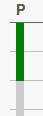
\includegraphics[width=0.05\textwidth]{img/progress.png}
  \end{center}
\end{wrapfigure}

Der Fortschrittsbalken soll anzeigen, bis zu welchem Punkt eine Datei
bereits bearbeitet worden ist.  Eine \textbf{grüne} Markierung zeigt
den bereits bearbeiteten Bereich an, während der Balken ansonsten
\textbf{grau} hinterlegt ist.

Diese Markierung erfüllt derzeit folgende Funktionen:
\begin{itemize}
\item Wenn eine Datei geöffnet wird, springt der Editor automatisch an
  die Stelle, wo der Fortschrittsbalken endet.
\item Die automatische Lernfunktion lernt nur aus den Daten, die bereits grün
  markiert sind, und überschreibt nur Daten, die noch nicht grün markiert sind.
\end{itemize}

Wird eine Annotation an einem Token geändert, verlängert sich der
Fortschrittsbalken ggf.\ automatisch bis zu diesem Punkt.  Bedenken
Sie dies insbesondere, falls Sie einmal an eine spätere Stelle im Text
springen, um dort eine Annotation zu ändern!  Sie müssen sich in
diesem Fall merken, an welchem Punkt Sie zuvor gewesen sind, da die
Fortschrittsanzeige sich automatisch verlängert.

Durch Klick auf den Fortschrittsbalken kann dieser allerdings bei
Bedarf auch \textbf{manuell eingestellt} werden: Klick auf einen grünen Bereich
verkürzt den Balken bis zu diesem Punkt, Klick auf einen grauen
Bereich verlängert ihn entsprechend.


\subsubsection{Nummerierung}

\begin{wrapfigure}{r}{0.12\textwidth}
  \begin{center}\vspace{-2em}
    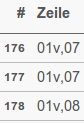
\includegraphics[width=0.1\textwidth]{img/zeile.png}
  \end{center}
\end{wrapfigure}

Zwei verschiedene Zeilennummern werden angezeigt:
\begin{enumerate}
\item Die interne Nummerierung (Spalte "`\#"') ist eine fortlaufende
  Zählung aller Token; über den Link "`Springe zu Zeile\ldots"' in der
  Navigationsleiste kann z.B.\ direkt zu einer bestimmten Zeilennummer
  gesprungen werden.
\item Die Spalte "`Zeile"' gibt die Zeilennummer in der
  Original-Transkription an. (In Einzelfällen, wenn ein Wort sich über
  mehrere Zeilen erstreckt, kann diese Angabe ungenau sein. Dies ist
  eine bekannte Einschränkung.)
\end{enumerate}

\subsubsection{Markierung von Problemfällen (E)}

\begin{wrapfigure}{r}{0.1\textwidth}
  \begin{center}\vspace{-2em}
    
\includegraphics[width=0.031\textwidth]{img/error.png}
  \end{center}
\end{wrapfigure}

Die Spalte "`E"' (ursprünglich für "`Error"') enthält eine Checkbox, in der
durch Anklicken eine rote Markierung gesetzt bzw.\ entfernt werden kann.  Diese
Markierung kann z.B.\ benutzt werden, um Fehler oder Problemfälle zu markieren,
die später noch einmal angesehen werden müssen.  Derart markierte Tokens lassen
sich später z.B.\ mithilfe der Suchfunktion gezielt auffinden.

\subsubsection{Token}

Es gibt zwei verschiedene Darstellungen der Wortformen, die annotiert
werden sollen: \textbf{Token~(Trans)} zeigt die
Original-Transkription, während \textbf{Token~(UTF)} eine
Unicode-Darstellung der Transkriptionszeichen enthält.  Es ist
möglich, den Editor so anzupassen, dass nur eine der beiden Formen
dargestellt wird -- siehe dazu Abschnitt~\ref{sec:anpassen}.

\subsubsection{POS- und Morphologie-Tags}

\begin{wrapfigure}{r}{0.35\textwidth}
  \begin{center}\vspace{-2em}
    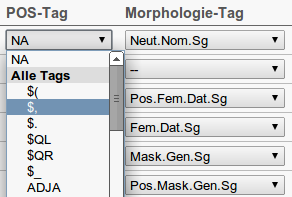
\includegraphics[width=0.3\textwidth]{img/pos.png}
  \end{center}
\end{wrapfigure}

Die Wortarten-Annotation in CorA erfolgt in zwei Schritten: zunächst
sollte über die entsprechende Dropdown-Box ein \textbf{POS-Tag}
ausgewählt werden; anschließend kann in der Spalte
\textbf{Morphologie-Tag} eine Kombination von morphologischen Angaben
ausgewählt werden.

Die Auswahlmöglichkeiten bei den Morphologie-Tags sind dabei
\textbf{abhängig vom gewählten POS-Tag}.  Falls der POS-Tag geändert
wird, und der aktuell selektierte Morphologie-Tag keine zulässige
Auswahl mehr für den neuen POS-Tag ist, so ändert CorA den
Morphologie-Tag \textbf{automatisch} auf einen zulässigen Wert.
Dieser wird natürlich in der Regel noch falsch sein!  Es ist daher
empfehlenswert, die beiden Spalten immer zusammen zu bearbeiten, bzw.\
nach Änderung des POS-Tags auch immer die morphologische Angabe zu
überprüfen.

Manchmal können die Dropdown-Boxen \textbf{rot umrandet} sein.  Dies
bedeutet, dass der entsprechende Tag auf jeden Fall fehlerhaft ist und
geändert werden sollte (z.B., wenn der Tagger nur "`?"' als Tag
vorgeschlagen hat).

\subsubsection{Lemmatisierung}

\begin{wrapfigure}{r}{0.35\textwidth}\vspace{-2em}
  \begin{center}
    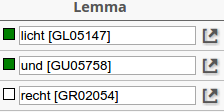
\includegraphics[width=0.28\textwidth]{img/1.2/lemma.png}\vspace{20px}
    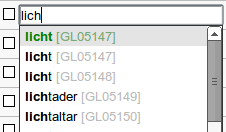
\includegraphics[width=0.28\textwidth]{img/lemma-edit.png}
  \end{center}
\end{wrapfigure}

Die Lemma-Spalte hat drei Bestandteile: eine \textbf{Checkbox}, um
Lemma-Einträge als "`bestätigt"' zu markieren; ein \textbf{Eingabefeld} für das
Lemma; und ggf.\ einen \textbf{Verweis} auf eine externe Resource (z.B.\
Online-Ausgabe eines Lexikons).

Das Eingabefeld ist mit einer \textbf{Dropdown-Liste mit
  Lemma-Vorschlägen} verknüpft.  Diese Liste öffnet sich automatisch,
sobald eine Eingabe in dem Feld gemacht wird (s.~Abbildung rechts).
Alternativ lässt sie sich auch durch Doppelklick in das Eingabefeld
oder mit "`Pfeiltaste nach unten"' öffnen.  Die Liste kann
verschiedene Arten von Einträgen enthalten:
\begin{enumerate}
\item \textbf{Grau hinterlegte} Einträge sind automatisch generierte
  Vorschläge.
\item Zusätzlich \textbf{grün hervorgehobene} Einträge sind Lemmata,
  die an anderer Stelle für eine gleichlautende Wortform bereits
  eingetragen und als "`bestätigt"' markiert wurden.  Diese Vorschläge
  werden aus allen Texten im selben Projekt generiert.
\item Alle anderen Einträge sind durch Autovervollständigung gefundene Treffer in einer verlinkten Lemma-Liste (nur, falls eine solche Liste für das Projekt definiert worden ist). Dabei gilt:
  \begin{enumerate}
  \item es wird immer nur nach passendem Wortanfang gesucht;
  \item Diakritika werden ignoriert, d.h.\ Eingabe von
    \emph{geta} findet sowohl \emph{getacht} wie auch \emph{getäckel}
    oder \emph{getâkel}; und
  \item wenn es sehr viele Treffer gibt, wird nur ein Teil davon
    angezeigt, d.h.\ befindet sich der gesuchte Eintrag nicht in der
    Liste, müssen Sie evtl.\ weitere Buchstaben dazu eingeben.
  \end{enumerate}
\end{enumerate}

Durch Anklicken eines Eintrags in der Liste wird dieser in das
Eingabefeld übernommen (alternativ: Auswählen mit den Pfeiltasten und
Drücken der "`Tabulator"'-Taste).  Das Textfeld akzeptiert aber auch
beliebige andere Eingaben; es muss nicht zwingend ein Eintrag aus der
Liste übernommen werden!

Die \textbf{Checkbox für "`bestätigte"' Lemmata} wird automatisch markiert,
wenn ein grün hervorgehobener Eintrag aus der Liste ausgewählt wird.
Ebenso wird eine Markierung automatisch wieder entfernt, wenn der
Lemma-Eintrag auf andere Weise geändert wird.  Dies soll vor
unabsichtlichen Fehlern (und damit vor falschen Einträgen, die
trotzdem "`bestätigt"' sind) schützen.

Klicken auf das
Symbol 
\includegraphics[height=\baselineskip]{img/1.2/lemma-link.png} öffnet eine
evtl.\ verlinkte externe Resource in einem separaten Browserfenster.  Dabei wird
automatisch der zu dem eingetragenen Lemma passende Eintrag aufgerufen.  Weitere
Aufrufe öffnen sich immer in demselben Fenster.
% , sodass CorA- und
% Grimm-Browserfenster auch gut nebeneinander platziert werden können,
% wenn öfter in Grimm nachgeschlagen werden soll.

\subsubsection{Normalisierung \& Modernisierung}

\begin{wrapfigure}{r}{0.45\textwidth}%\vspace{-2em}
  \begin{center}
    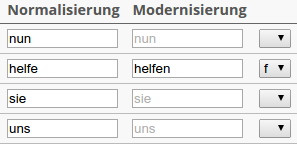
\includegraphics[width=0.38\textwidth]{img/1.2/norm.png}
  \end{center}
\end{wrapfigure}

Die Spalten ``Normalisierung'' und ``Modernisierung'' sind einfache Textfelder,
die beliebige Eingaben akzeptieren.  Falls die Spalte ``Modernisierung'' leer
ist, erscheint standardmäßig der Wert der Normalisierung grau hinterlegt.  Dies
spiegelt die Konvention wider, dass die Modernisierung nur angegeben werden
muss, wenn sie sich von der Normalisierung unterscheidet.

In der Dropdown-Box neben dem Modernisierungsfeld kann der Typ der
Modernisierung (z.B.\ ``f''~= ``durch Flexion bedingt'', ``s''~= ``durch
Semantik bedingt'') näher spezifiziert werden.  Ist die Modernisierung leer,
bleibt diese Dropdown-Box deaktiviert; wird in das Modernisierungsfeld etwas
eingetragen, so muss auch ein Wert in der Dropdown-Box ausgewählt werden.
Andernfalls wird sie rot umrandet dargestellt, um auf die fehlende Annotation
hinzuweisen.

\subsubsection{Kommentarfeld}

Die Spalte "`Kommentar"' enthält ein Eingabefeld, worin ein beliebiger
Freitext eingegeben werden kann.  Diese Kommentare sind unabhängig von
etwaigen Kommentaren in der Transkription (z.B.\ +K~\ldots{}~@K).

\subsubsection{Kontextmenü}

\vspace{-.5em} Klicken auf den
Pfeil 
\includegraphics[height=\baselineskip]{img/dropdown.png} öffnet
ein Kontextmenü.  Derzeit besteht es aus folgenden Einträgen:

\begin{itemize}
\item \textbf{``Suche ähnliche\ldots''} öffnet den Suchdialog mit voreingestellten Werten (vgl.\ Abs.~\ref{sec:sufu});
\item \textbf{``Token bearbeiten\ldots'', ``Token hinzufügen\ldots''} und \textbf{``Token löschen''} ermöglichen die Bearbeitung der Original-Transkription, welcher der Abschnitt~\ref{sec:bearbeiten} gewidmet ist.
\end{itemize}

\newpage
\subsection{Die Toolbar}

Am oberen Rand des Editors befindet sich eine Toolbar, die zur Navigation
innerhalb des Dokuments und zum Aufrufen verschiedener Funktionen verwendet
werden kann.

\begin{figure}[!h]
  \centering
  \begin{overpic}[width=\linewidth]{img/1.2/editor-toolbar.png}
    \put(1.5,3){\circled{1}}
    \put(13.25,3){\circled{2}}
    \put(18,3){\circled{3}}
    \put(34.75,3){\circled{4}}
    \put(40.25,3){\circled{5}}
    \put(53.25,3){\circled{6}}
    \put(60.25,3){\circled{7}}
    \put(87,3){\circled{8}}
  \end{overpic}
  \caption{Die Editor-Toolbar}
  \label{fig:editor-toolbar}
\end{figure}

\begin{enumerate}[label=\protect\circled{\arabic*}]
\item Zeigt die \textbf{aktuelle Seitenzahl} und die Gesamtanzahl an Seiten an.  Durch Klick auf dieses Element kann direkt zu einer bestimmten Seite im Editor navigiert werden.
\item \textbf{Blättert} eine Seite vor bzw.\ zurück.
\item Springt zu einer bestimmten Zeile innerhalb des Dokuments.
\item Macht die letzte Änderung \textbf{rückgängig} bzw.\ \textbf{stellt sie wieder her.}
\item Aktiviert die \textbf{Suchfunktion} (vgl.\ Abs.\ \ref{sec:sufu}).
\item Springt zum vorherigen bzw.\ nächsten Suchergebnis.  Nur aktiv, wenn zuvor eine Suche ausgeführt wurde.
\item Startet die \textbf{automatische Annotation} mithilfe externer Tools (vgl.\ Abs.\ \ref{sec:autoanno}).
\item Zeigt die \textbf{Metadaten} des aktuellen Dokuments an bzw.\ erlaubt, sie zu ändern.
\end{enumerate}

Zeilen- und Seitenzahlen beziehen sich dabei immer auf die Darstellung im
Editor, \textbf{nicht} auf Zeilen bzw.\ Seiten in der Transkription!  Die
Seitenzahlen sind abhängig davon, wieviele Zeilen pro Seite angezeigt werden,
was vom Benutzer selbst eingestellt werden kann (vgl.\
Abschnitt~\ref{sec:anpassen}).  Daher können sie auch für denselben Text von
Benutzer zu Benutzer verschieden sein!

Funktionen zum Navigieren anhand der Nummerierung in der Original-Transkription
sind momentan noch nicht implementiert.

\newpage
\subsection{Suchen innerhalb des Dokuments}
\label{sec:sufu}

Durch Klick auf ``Suchen...'' im Editor oder ``Suche ändern'' in den
Suchergebnissen kann eine neue Suche gestartet werden.  CorA kann nur im aktuell geöffneten Dokument suchen, und nur nach einzelnen Wortformen -- eine kontextabhängige Suchanfrage (z.B.\ ``Token \emph{x} gefolgt von \emph{y}'') ist nicht möglich.

\begin{figure}[!h]
  \centering
  \begin{overpic}[width=0.6\linewidth]{img/1.2/such-dialog.png}
    \put(30,27){\circled{1}}
    \put(2,16){\circled{2}}
    \put(90,22){\circled{3}}
    \put(20.5,6){\circled{4}}
    %\put(94,6){\circled{5}}
  \end{overpic}
  \caption{Suchfenster}
  \label{fig:sufu}
\end{figure}

Folgende Einstellungen können bei der Suche vorgenommen werden:

\begin{enumerate}[label=\protect\circled{\arabic*}]
\item Steuert, ob \textbf{alle} oder nur \textbf{mindestens eins} der angegebenen Suchkriterien erfüllt sein müssen.
\item Definiert die Suchkriterien, d.h.\ welches \textbf{Feld} (z.B.\ Token, POS-Tag) auf welche Weise (z.B.\ ``ist'', ``endet auf'') mit welchem \textbf{Wert} verglichen werden soll.
\item Entfernt ein Suchkriterium bzw.\ fügt ein neues hinzu.
\item Löscht alle momentan angegebenen Suchkriterien.
\end{enumerate}

Die Suchergebnisse werden in einem separaten Tab ``Suchen'' angezeigt.  Annotationen können hier genauso bearbeitet werden wie im Haupteditor auch:

\begin{figure}[!h]
  \centering
  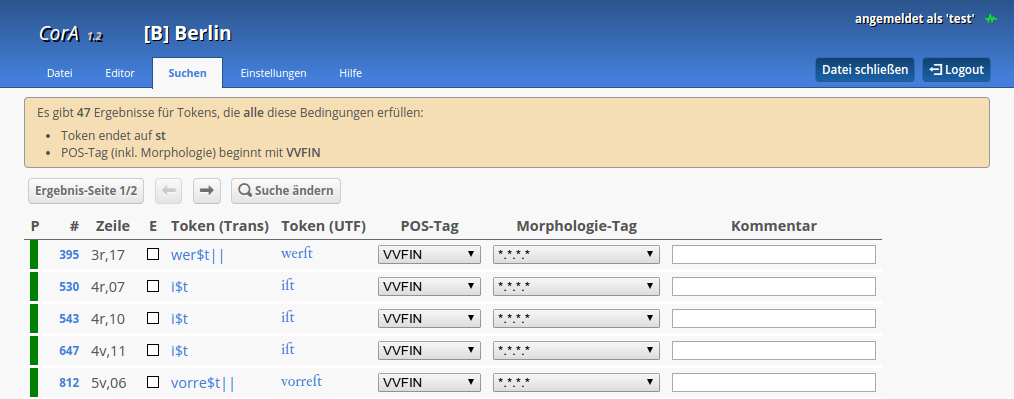
\includegraphics[width=\linewidth]{img/1.2/such-tab2.png}
  \caption{Anzeige der Suchergebnisse}
  \label{fig:such-tab}
\end{figure}

Ein Klick auf die Zeilennummer oder das Token \textbf{springt zur entsprechenden Textstelle im Editor}.  Sie können durch Klick auf den jeweiligen Tab jederzeit zwischen Editor und Suchergebnissen hin und her wechseln.  Zum Navigieren innerhalb der Suchergebnisse können außerdem die entsprechenden Buttons im Editor (\circled{6} in Abb.~\ref{fig:editor-toolbar}) verwendet werden.

Um eine neue Suche zu starten, klicken Sie einfach wieder auf ``Suchen\ldots'' bzw.\ ``Suche ändern''.  Ihre letzten Suchkriterien bleiben erhalten, bis Sie im Suchfenster auf ``Zurücksetzen'' klicken, sodass Sie z.B.\ auch ihre vorherige Suche modifizieren oder erneut ausführen können.

\begin{infobox}{}
  Beachten Sie, dass die Suchergebnisse sich \textbf{nicht} automatisch aktualisieren, wenn Sie zwischenzeitlich Änderungen im Editor vornehmen.  Wenn Sie also z.B.\ nach Tokens mit dem POS-Tag \emph{XX} suchen, und anschließend bei einigen Tokens den POS-Tag \emph{XX} auf \emph{YY} ändern, werden diese dennoch weiterhin in den Suchergebnissen angezeigt.  Sie können jedoch einfach das Suchfenster öffnen und die Suche mit denselben Kriterien erneut starten, um die Ergebnisse zu aktualisieren.
\end{infobox}

Um nach Tokens zu suchen, die einem bestimmten Token in der Editor-Ansicht
ähnlich sind, gibt es im \textbf{Dropdown-Menü} des jeweiligen Tokens den
Eintrag \textbf{``Suche ähnliche\ldots''}.  Dieser Menüpunkt öffnet das
Suchfenster, wobei die Suchkriterien automatisch so ausgefüllt sind, dass sie
den Annotationen des aktuell ausgewählten Tokens entsprechen.  Die Suche kann
entweder direkt ausgeführt oder noch weiter modifiziert werden.

\newpage
\subsection{Automatische Annotation mit externen Tools}
\label{sec:autoanno}

CorA bietet die Möglichkeit, direkt aus der Weboberfläche heraus externe
Annotationstools aufzurufen.  Hierzu klicken Sie in der Editor-Ansicht auf den
Knopf ``Automatisch annotieren'' (vgl.\ \circled{7} in
Abb.~\ref{fig:editor-toolbar}); es sollte sich ein Fenster ähnlich wie dieses
öffnen:

\begin{figure}[!h]
  \centering
  \begin{overpic}[width=0.5\linewidth]{img/1.2/anno-dialog.png}
    %\put(94,6){\circled{5}}
  \end{overpic}
  \caption{Starten der automatischen Annotation}
  \label{fig:autoanno}
\end{figure}

Hier können Sie zwischen verschiedenen Taggern auswählen, die auf das aktuell
geöffnete Dokument anwendbar sind.  Die Einrichtung dieser Tagger kann nur ein
Administrator vornehmen; bitte fragen Sie ggf.\ dort nach, wenn Sie sich nicht
sicher sind, was ein bestimmter Tagger in der Auswahlliste genau macht, oder
falls ein neuer Tagger hinzugefügt werden soll.

Durch Klick auf \textbf{``Annotieren''} wird der Tagger aufgerufen und auf das
aktuell geöffnete Dokument angewendet; dabei werden alle eventuell bereits
bestehenden Annotationen \textbf{überschrieben,} die \textbf{nicht} mittels des
Fortschrittsbalkens grün markiert sind.

\begin{alertbox}{}
  Das automatische Annotieren kann \textbf{nicht rückgängig} gemacht werden!
  Bitte stellen Sie vor dem Klick auf ``Annotieren'' sicher, dass der grüne
  Fortschrittsbalken an der korrekten Position steht.
\end{alertbox}

Der Button \textbf{``Neu trainieren''} ist je nach Konfiguration nicht für jeden
Tagger verfügbar.  Falls er aktiv ist, wird hierdurch der ausgewählte Tagger auf
dem geöffneten Text \textbf{und allen Texten des übergeordneten Projekts} neu
trainiert.  Hierfür werden \textbf{nur} Textpassagen herangezogen, die mittels
des Fortschrittsbalkens grün markiert sind.

\newpage
\subsection{Anpassen des Editors}
\label{sec:anpassen}

% Die \textbf{Anordnung der Spalten} kann per "`Drag \& Drop"' geändert
% werden.  Gehen Sie dazu auf eine beliebige Spalten-Überschrift,
% klicken und halten Sie die linke Maustaste gedrückt, ziehen Sie die
% Spalte an eine beliebige andere Position, und lassen die Maustaste
% wieder los.  CorA merkt sich die individuelle Anordnung der Spalten
% automatisch.

Der Editor kann über den \textbf{Reiter "`Einstellungen"'} individuell angepasst
werden (s.\ Abbildung~\ref{fig:settings}).

Die Einstellung \textbf{``Zeilen pro Seite''} steuert, wieviele Wortformen im
Editor gleichzeitig dargestellt werden.  Wir empfehlen, aus Performance-Gründen
nicht mehr als 50~Zeilen pro Seite anzeigen zu lassen.  \textbf{``Überlappende
  Zeilen''} gibt an, wieviele Zeilen vom Seitenende auch noch auf dem Anfang der
nächsten Seite erscheinen sollen.  Beide Einstellungen müssen durch Klick auf
"`Zeilen-Einstellungen übernehmen"' bestätigt werden.

\textbf{``Sichtbare Spalten''} steuert, welche Spalten im Editor angezeigt
werden.  Standardmäßig sind alle Spalten sichtbar, durch Abwählen einzelner
Checkboxen können bestimmte Spalten jedoch ausgeblendet werden.  Dies kann der
besseren Übersichtlichkeit im Editor dienen.  Änderungen hier sind sofort
wirksam.

\begin{figure}[tb]
  \centering
  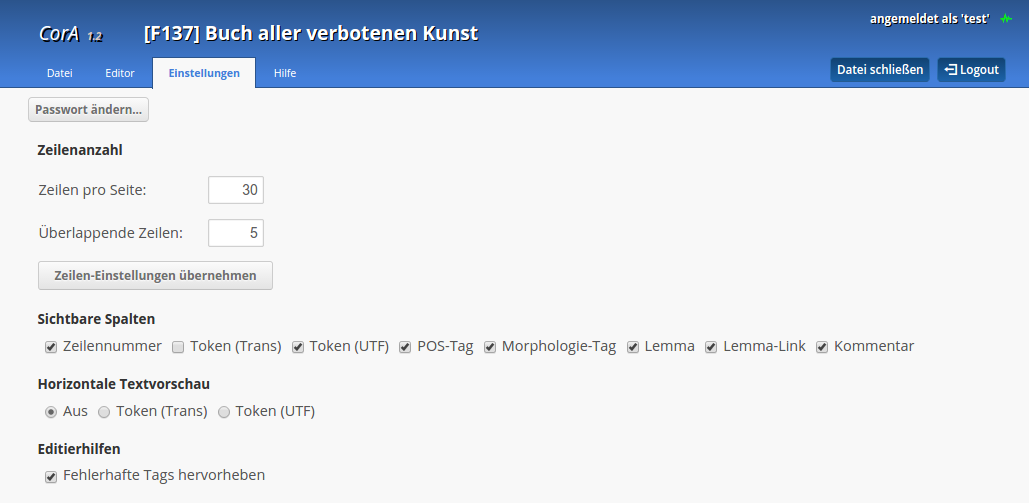
\includegraphics[width=\linewidth]{img/1.2/einstellungen.png}
  \caption{Der Reiter "`Einstellungen"'}
  \label{fig:settings}
\end{figure}

Unter \textbf{``Horizontale Textvorschau''} kann eingestellt werden, welche Tokenebene (Trans oder UTF) in der Textvorschau am unteren Bildschirmrand angezeigt werden soll.  Alternativ kann die Textvorschau hier auch deaktiviert werden.

Die Option \textbf{``Fehlerhafte Tags hervorheben''} steuert, ob
fehlerhafte Tags im Editor mit einer roten Umrandung versehen werden.

\newpage
\section{Bearbeiten der Transkription}
\label{sec:bearbeiten}

CorA ist in erster Linie ein Annotationstool, stellt jedoch auch
Funktionen für den Fall bereit, dass Änderungen an der
Original-Transkription vorgenommen werden müssen.  Die dafür nötige
Vorgehensweise kann anfangs -- je nach Art der Änderung --
möglicherweise etwas unintuitiv sein.  Dies ist zumeist dann der Fall,
wenn die Änderungen sich auf die Tokenisierung auswirken (z.B.\ wenn
zwei Wortformen, die in CorA auf zwei Zeilen verteilt sind,
zusammengezogen werden sollen).  Im Folgenden werden die einzelnen
Funktionen beschrieben und an einigen praktischen Beispielen
erläutert.

\begin{alertbox}{Wichtig!}
  \begin{itemize}\vspace{-1.5em}
  \item Änderungen an der Transkription können \textbf{nicht rückgängig} gemacht
    werden!  Sie können die Transkription zwar per Hand wieder zurück ändern, es
    gibt jedoch keine Möglichkeit, den Zustand der Transkription vor der
    Bearbeitung zu sehen.
  \end{itemize}
\end{alertbox}

Durch Klick auf das
Symbol 
\includegraphics[height=\baselineskip]{img/dropdown.png}
(standardmäßig ganz am Ende jeder Zeile) öffnet sich ein Kontextmenü,
worüber alle Funktionen zum Ändern der Transkription aufgerufen werden
können:

\begin{center}
  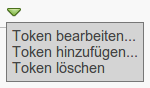
\includegraphics[width=0.25\linewidth]{img/dropdown-menu.png}
\end{center}

Die Funktion "`Token bearbeiten"' kann außerdem aufgerufen werden
durch \textbf{Doppelklick} auf die entsprechende Wortform in der
Spalte "`Token~(Trans)"' oder "`Token~(UTF)"'.

\subsection{Token bearbeiten}
\label{sec:trans-edit}

\begin{figure}
  \centering
  \begin{subfigure}[b]{0.4\textwidth}
    \centering
    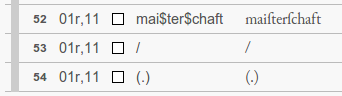
\includegraphics[width=\textwidth]{img/trans-bsp1.png}
    \caption{}
    \label{fig:trans-bsp1}
  \end{subfigure}
  \hfill
  \begin{subfigure}[b]{0.4\textwidth}
    \centering
    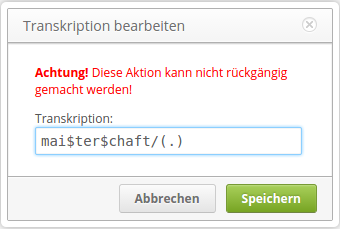
\includegraphics[width=\textwidth]{img/1.2/trans-edit1.png}
    \caption{}
    \label{fig:trans-edit1}
  \end{subfigure}
  \caption{Bearbeiten der Original-Transkription}
  \label{fig:trans-edit}
\end{figure}

Für die Bearbeitung der Transkription ist es wichtig zu verstehen,
dass die Zeilen im Editor und die Transkription, die bearbeitet wird,
sich nicht immer 1:1 entsprechen.  Dies lässt sich am besten an einem
Beispiel erläutern: Abbildung~\ref{fig:trans-bsp1} zeigt einen
Ausschnitt von drei Zeilen aus dem Editor;
Abbildung~\ref{fig:trans-edit1} zeigt das Fenster, das sich öffnet,
wenn eine beliebige dieser drei Zeilen bearbeitet wird.  Die
Transkription \trans{mai\$ter\$chaft/(.)} wird für die Annotation in
die drei separaten Token \trans{mai\$ter\$chaft}, \trans{/} und
\trans{(.)} zerlegt, während die Bearbeitung dieser Transkription
jedoch als Ganzes erfolgt.

Im Editorfenster aus Abbildung~\ref{fig:trans-edit1} können nun
beliebige Änderungen vorgenommen werden, die nach einem Klick auf
"`Speichern"' übernommen werden.  Für alle Änderungen gilt, dass diese
zunächst mit Hilfe des Check-Skripts geprüft werden.  Ungültige
Transkriptionszeichen werden von CorA nicht akzeptiert; die
entsprechende Fehlermeldung des Check-Skripts wird dann angezeigt und
die Änderung wird nicht vorgenommen.

% \textbf{Leerzeichen in der Transkription} haben an dieser Stelle eine
% besondere Bedeutung.  Sie werden von CorA immer dann verwendet, wenn
% sich ein Token in der Original-Transkription über mehrere Zeilen
% erstreckt:

% \begin{quote}\ttfamily\small
%   F137-02r,20~~~~dein hoche vernunft \$o begirlich be=\\
%   F137-02r,21~~~~gert(,) \$u\*cht vnd erfra\textbackslash{}vgt(,) alle kun\$t
% \end{quote}

% Das Token, das sich hier über beide Zeilen erstreckt, würde beim
% Bearbeiten in CorA als \trans{be=~gert(,)} angezeigt.  Das Leerzeichen
% markiert dabei die Stelle, an der der Zeilenumbruch stattfindet.
% Dieses Leerzeichen darf beim Bearbeiten der Transkription nicht
% entfernt werden, da ansonsten der hintere Teil in der
% Original-Transkription mit auf die vorherige Zeile gezogen würde!

% Andersherum dürfen Leerzeichen beim Bearbeiten der Transkription nur
% dann eingefügt werden, wenn Sie einen Zeilenumbruch repräsentieren
% sollen.  Dies ist nur möglich, wenn das bearbeitete Token am Ende
% einer Zeile steht und wird ansonsten von CorA nicht akzeptiert.
% Außerdem muss jedem Leerzeichen ein Trennzeichen vorausgehen.

% \begin{infobox}{Tipp}
%   Möchten Sie einmal in die Transkription tatsächlich ein Leerzeichen
%   einfügen, das nicht für einen Zeilenumbruch steht (z.B.\ um
%   \trans{in\#der} in \trans{in der} abzuändern), so sind dafür mehrere
%   Schritte nötig!  In Abschnitt~\ref{sec:trans-bsp} wird dies an
%   Beispielen verdeutlicht.
% \end{infobox}

\subsection{Token hinzufügen}

\begin{figure}
  \centering
  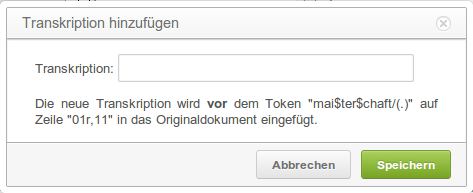
\includegraphics[width=0.6\linewidth]{img/trans-add.png}
  \caption{Hinzufügen eines Tokens}
  \label{fig:trans-add}
\end{figure}

Wählen Sie "`Token hinzufügen\ldots"' aus dem Kontextmenü aus, um eine
neue Transkription \textbf{vor} einem bestehenden Token einzufügen.
Es öffnet sich ein Fenster, worin die neue Transkription eingegeben
werden kann (s.\ Abbildung~\ref{fig:trans-add}).  Dabei gelten
dieselben Regeln wie für das Bearbeiten einer Transkription (siehe
oben).

In einem Hinweistext unter dem Eingabefeld wird nochmals erläutert, an
welcher Position und auf welcher Zeile der Original-Transkription das
neue Token eingefügt wird.  Überprüfen Sie diese Angaben in jedem
Fall, um sicherzustellen, dass Sie das Token an der richtigen Stelle
im Text einfügen!

\subsection{Token löschen}

Wählen Sie "`Token löschen"' aus dem Kontextmenü aus, um eine
Transkription komplett aus dem Text zu löschen.  Sie müssen diese
Aktion zur Sicherheit immer bestätigen, da auch das Löschen eines
Tokens nicht rückgängig gemacht werden kann.  In dem entsprechenden
Hinweisfenster können Sie außerdem nochmals überprüfen, welche
Transkription bei einem Bestätigen der Aktion tatsächlich gelöscht
wird.

\subsection{Praktische Beispiele}
\label{sec:trans-bsp}

Für Änderungen in der Transkription, die Einfluss auf die
Tokenisierung haben, können mitunter mehrere Bearbeitungsschritte
notwendig sein.  Daher werden hier einige Beispiele gegeben, wie die
Transkription in diesen Fällen geändert werden kann.

\paragraph{Beispiel 1.}  Angenommen, ein Token in der Transkription
soll (durch Einfügen eines Leerzeichens) in zwei Token aufgetrennt
werden.  Ein Beispiel wäre die Änderung von \trans{in\#der} zu
\trans{in der}.  Hierzu sind zwei Schritte nötig:
\begin{enumerate}
\item Gehen Sie auf die Zeile mit der Transkription \trans{in\#der},
  öffnen Sie das Kontextmenü
  (
\includegraphics[height=\baselineskip]{img/dropdown.png}), und
  wählen Sie "`Token hinzufügen"'.  Fügen Sie jetzt \trans{in} als
  neue Transkription ein.\\$\to$ In der Transkription steht jetzt
  \trans{in in\#der}.
\item Doppelklicken Sie nun auf die Transkription \trans{in\#der} und
  ändern Sie sie ab zu \trans{der}.\\$\to$ In der Transkription steht
  jetzt \trans{in der}.
\end{enumerate}

\paragraph{Beispiel 2.}  Angenommen, zwei Token in der Transkription
sollen zu einem zusammengefügt werden.  Beispielsweise soll
\trans{zu~vor} geändert werden in \trans{zu\#vor}.  Dies ist der
umgekehrte Fall zu Beispiel~1.  Hierfür sind ebenfalls wieder zwei
Schritte nötig:
\begin{enumerate}
\item Doppelklicken Sie auf die Transkription \trans{vor} und ändern
  Sie sie ab zu \trans{zu\#vor}.\\$\to$ In der Transkription steht
  jetzt \trans{zu~zu\#vor}.
\item Gehen Sie nun auf die Zeile mit der Transkription \trans{zu},
  öffnen Sie das Kontextmenü, und wählen Sie "`Token löschen"'.\\$\to$
  In der Transkription steht jetzt \trans{zu\#vor}.
\end{enumerate}

\begin{infobox}{Tipp}
  Seien Sie besonders vorsichtig, wenn sie eine Transkription
  bearbeiten, die sich über mehrere Zeilen erstreckt!  Angenommen, in
  der folgenden Original-Transkription sollen die ersten beiden Token
  zu \trans{MVLLNER\#ORD=~nung} zusammengefügt werden:

  \begin{quote}\ttfamily\small
    F57-1r,01~~~~MVLLNER ORD=\\
    F57-1r,02~~~~nung in den Für\$tlichen Thiroli\$chen Stet=
  \end{quote}

  Dies kann wie oben beschrieben erreicht werden, indem Sie in CorA
  zunächst das Token \trans{ORD=~nung} abändern in
  \trans{MVLLNER\#ORD=~nung}, und anschließend das erste Token
  \trans{MVLLNER} löschen.

  Andersherum ist es jedoch \textbf{nicht} möglich, zuerst \trans{MVLLNER} in
  \trans{MVLLNER\#ORD=~nung} zu ändern und dann das Folgetoken zu löschen!  Die
  entsprechende Operation wird fehlschlagen, da sich die neue Transkription
  nicht am Zeilenende befindet.

  Behelfen Sie sich \textbf{in keinem Fall}, indem Sie den Zeilenumbruch
  weglassen!  Das Ergebnis würde dann fälschlicherweise so interpretiert\ldots{}

  \begin{quote}\ttfamily\small
    F57-1r,01~~~~MVLLNER\#ORD=nung\\
    F57-1r,02~~~~in den Für\$tlichen Thiroli\$chen Stet=
  \end{quote}

  \ldots{}was vermutlich nicht Ihrer Absicht entspricht.
\end{infobox}

\paragraph{Beispiel 3.}  Angenommen, ein fälschlich gesetztes
Trennzeichen am Zeilenende soll entfernt werden.  Beispielsweise soll
\trans{in(=)~der} zu \trans{in~der} geändert werden, wobei die beiden
Wortformen auf verschiedenen Zeilen in der Transkription stehen.  Dies
kann mit folgenden Schritten realisiert werden:
\begin{enumerate}
\item Gehen Sie auf die erste Zeile \textbf{nach} der Transkription
  \trans{in(=)~der}, öffnen Sie das Kontextmenü, und wählen Sie
  "`Token hinzufügen"'.  Fügen Sie jetzt \trans{der} als neue
  Transkription ein.\\$\to$ In der Transkription steht jetzt
  \trans{in(=)~der~der}.
\item Doppelklicken Sie nun auf die Transkription \trans{in(=)~der}
  und ändern Sie sie zu \trans{in}.\\$\to$ In der Transkription steht
  jetzt \trans{in~der}.
\end{enumerate}

\paragraph{Beispiel 4.}  Angenommen, das Token \trans{ge} am Ende
einer Zeile soll mit dem ersten Token \trans{schah} der nächsten Zeile
mittels eines Trennstriches \trans{(=)} zusammengeführt werden.  Dies
gelingt mit folgenden Schritten:
\begin{enumerate}
\item Doppelklicken Sie auf die Transkription \trans{ge} und ändern Sie sie zu
  \trans{ge(=)~schah} (mit Zeilenumbruch zwischen den Wörtern).
\item Löschen Sie nun einfach das zweite \trans{schah}.
\end{enumerate}

\vspace{2em} %% HACK
\section{Tastaturbefehle}

Mit \textbf{Tab} (Tabulator-Taste) springen Sie im Editor zum nächsten
editierbaren Feld, mit \textbf{Shift+Tab} springen Sie ein Feld
zurück.  (Dies ist eine Funktion Ihres Internetbrowsers, nicht von
CorA selbst.)

In den Dropdown-Menüs für POS- und Morphologie-Tags können Sie mit
\textbf{Pfeiltaste nach oben/unten} zwischen den Tags wechseln.
Dasselbe gilt für das Menü mit den Lemma-Vorschlägen.  Alternativ
können Sie auch die Anfangsbuchstaben des gewünschten Tags eingeben.
(Dies ist eine Funktion Ihres Internetbrowsers, nicht von CorA
selbst.)

Innerhalb von Textfeldern (außer Lemma) können die \textbf{Pfeiltasten nach
  oben/unten} außerdem zum Navigieren zwischen den Zeilen benutzt werden.

Mit \textbf{Strg+F} öffnet sich das Suchfenster (s.\ Abs.\ \ref{sec:sufu}).

\newpage
\section{Umgang mit Fehlermeldungen}
\label{sec:error}

\begin{figure}
  \centering
  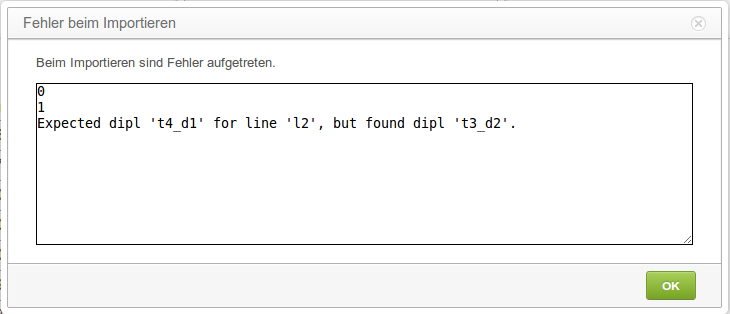
\includegraphics[width=0.8\linewidth]{img/import-error.png}
  \caption{Eine Fehlermeldung beim Import}
  \label{fig:import-error}
\end{figure}

Trotz aller Bemühungen können wir leider nicht ganz ausschließen, dass
während der Benutzung von CorA auch Fehlermeldungen auftreten.  In
unvorhergesehenen Fällen können diese Meldungen mitunter recht
kryptisch sein; Abbildung~\ref{fig:import-error} zeigt ein Beispiel
für eine (hoffentlich niemals auftretende\ldots) Fehlermeldung beim
Importieren einer Datei.  Damit wir in so einem Fall das
zugrundeliegende Problem so schnell wie möglich beheben können, bitten
wir Sie darum, ein paar einfache Hinweise zu beachten.

\begin{enumerate}
\item Melden Sie Fehler immer per \textbf{E-Mail} an \mmb{}.
\item Melden Sie uns Fehler, die Sie sich nicht erklären können, bitte
  in jedem Fall!  Wir können nur Fehler beheben, von denen wir auch
  wissen.
\item Senden Sie uns eine \textbf{aussagekräftige} Beschreibung des
  Fehlers! Dazu sollten immer folgende Informationen gehören:
  \begin{itemize}
  \item Was genau haben Sie unmittelbar vor dem Auftreten des Fehlers
    getan? (z.B.\ \emph{auf den Knopf "`Datei speichern"' geklickt})
  \item Wie genau äußert sich der Fehler? Falls es eine Fehlermeldung
    gibt: bitte die komplette Meldung kopieren und einfügen!
  \item An welcher Datei oder welchem Token genau haben Sie
    gearbeitet, als der Fehler auftrat? Falls der Fehler beim
    Importieren auftritt: die Datei, die importiert werden sollte, als
    Anhang mitschicken!
  \end{itemize}
\end{enumerate}

\end{document}
